\chapter{基于国产AI处理器的Top-k算法测试验证}

本章首先介绍了Topk-k算子测试用到的实验环境,同时也描述了整个算子测试的流程。
接着自行编写脚本生成大量的测试用例,用于测试自实现 Top-k 算子的准确度是否满足要求,
以确认功能是否正确。
然后测试了不同输入规模下,Topk 算子相对于全排序Top-k算子 和 Nvidia芯片上Top-k算子的性能表现情况。
最后将自实现
 Top-k 算子集成在Pytorch深度学习框架中,对目前比较流行的模型进行训练,
 并通过检测结果验证了Top-k 算子的可用性。

\section{实验环境与测试流程}
\subsection{实验环境}

测试的环境配置如表~\ref{tab:peizhi}所示。
\begin{table}[h]
    \centering
    \caption{表 5.1 硬件环境配置}
    \begin{tabular}{|l|l|}
    \hline
    类型 & 配置信息 \\
    \hline
    AI处理器 & DLP-M处理器 \\
    \hline
    CPU & Intel Xeon Silver 4114 \\
    \hline
    Nvidia GPU & A100-40G \\
    \hline
    操作系统 & CentOS - 7 \\
    \hline
    开发语言 & BC 4.7.0, C++11, Python 2.7.5 \\
    \hline
    编译器 & CC 4.7.1, gcc 4.8.5 \\
    \hline
    \end{tabular}
    \label{tab:peizhi}
    \end{table}
    
    本次实验以 CPU+国产AI 处理器(以下简称 MLU)异构编程模式进行,用到了BC、C++ 以及 Python 
    三种编程语言。BC 编程语言用于实现 MLU 端的 Top-k 算法计算过程;
    C++ 编程语言则用于实现 CPU 端的数据准备;
    Python 编程语言用于 编写测例用例生成脚本。
    CC(Compiler Collection,BC 语言编译器)是基于 Clang和 LLVM 开发的 BC 编译器主驱动程序
    ,负责将 BC 源码文件编译为 MLISA 汇编文件。
    

\subsection{测试流程}
\begin{enumerate}
    \item 通过 RT 接口初始化设备,RT 包含设备管理、内存管理、任务队列管理、 设备端程序执行、通知管理等功能,使用 BC 编写的程序需要借助于 RT 提供的 接口才能运行在 MLU 设备上。
    \item 初始化 HOG 描述符,并为保存 HOG 参数内容的结构体创建一个句柄。 同时计算出当前输入参数下计算得到的 HOG 特征向量需要占用的内存空间大 小, 并分配对应的内存空间。
    \item 准备输入数据,调用 RT 接口分配设备内存,并将输入数据拷贝到设备 内存中。
    \item MLU 端调用自实现的 HOG 算子,得到 HOG 特征向量。CPU 端调用 RT接口等待任务队列执行完成。
    
    \item 调用RT接口将Top-k算子的计算结果复制到主机侧。
    \item 主机侧调用Top-k的串行实现,得到比对的计算结果。
    \item 将设备端的计算结果与主机端的计算结果进行比较。
    \item 调用RT接口,释放主机端和设备端的内存以及任务队列等资源。
    
\end{enumerate}
整个计算流程如图~\ref{fig:test}所示:

\begin{figure}[ht]
    \centering
    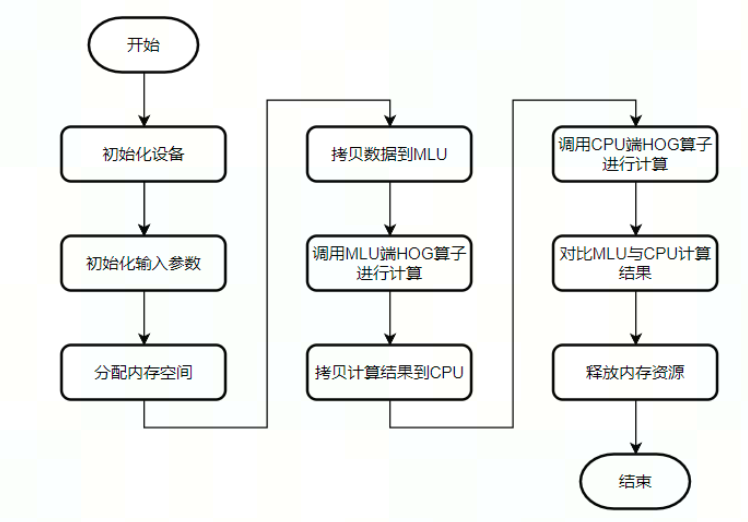
\includegraphics[width=1.0\textwidth]{test.png}
    \caption{RadixSelect测试流程图}
    \label{fig:test}
    % \note{注:图注的内容不宜放到图题中。}
\end{figure}


\section{Top-k算子功能测试}
在完成深度学习处理器的Top - K算子实现后,便可以开展算子的功能性与性能验证工作。
首先是功能验证,其主要内容如下:
\begin{enumerate}
\item 对不同维度(dim)下Top-k查询结果的正确性进行验证。
\item 针对不同k值下的查询结果正确性进行验证。
\item 检验经largest排序后的数据返回是否正确。
\end{enumerate}

在进行Top-k正确性验证时,将计算结果与CPU计算结果进行对比,
误差计算公式见,其总mlu\_output表示设备端的计算结果,cpu\_output表示主机端使用CPU的计算结果。
    \begin{equation}
    \label{eq:diff1}
    diff1 = \frac{\sum \vert baseline - mlu \vert}{\sum \vert baseline \vert + \epsilon}
    \end{equation}
    
    \begin{equation}
    \label{eq:diff2}
    diff2 = \frac{\sum (baseline - mlu)^2}{\sum (baseline)^2 + \epsilon}
    \end{equation}
其中,diff1表示与CPU返回的Top-k计算结果的相对误差,
diff2表示与CPU返回的Top-k数据的均方差。
考虑到Top-k算子仅仅只是筛选类的算子,不在原数据上做具体的操作。因此diff1和diff2应当为0才能满足精度要求。
本部分主要展示输入数据的数据类型为float和int的误差。
\begin{table}
\centering
\caption{Top-k功能测试表}
\label{tab:presicion}
\begin{tabular}{cllll}
    \toprule
    数据规模         & k  & largest & diff1    & diff2 \\
    \midrule
    (10000) int& 100      & True      & 0.000000 & 0.000000 \\
    (1024,3000000)int & 10000 & False      & 0.000000 & 0.000000 \\
    (1,1000000,4,2)float   & 5000 & True      & 0.000000 & 0.000000 \\
    (1024,3,300,4,8)float & 300 & False      & 0.000000 & 0.000000 \\
    (100, 3, 30000, 4, 8)int & 20 & True      & 0.000000 & 0.000000 \\
    (1,1,1,10240000)float & 1000000 & False      & 0.000000 & 0.000000 \\

\bottomrule
\end{tabular}
\end{table}



\section{Top-k算子性能测试}

\section{Top-k算子可用性测试}

\section{本章小结}
